Η ρομποτική είναι η επιστήμη της αντίληψης και του χειρισμού του φυσικού κόσμου
μέσω συσκευών που ελέγχονται από υπολογιστές \cite{thrun2005probabilistic}.  Ως
επιστήμη συμβάλλεται από τους κλάδους του αυτομάτου ελέγχου, της επιστήμης των
υπολογιστών, των μαθηματικών, και ως πράξη από την επιστήμη της φυσικής, της
τεχνολογίας υλικών, της τεχνολογίας λογισμικού, και της ηλεκτρονικής. Το φυσικό
αντικείμενο της ρομποτικής είναι το ρομποτ: μία τεχνητή σύνθεση αντλούσα
πληροφορίες από το φυσικό περιβάλλον μέσω αισθητήριων συσκευών, επενεργούσα σε
αυτό μέσω φυσικών δυνάμεων, αποτελούμενη κατ' ελάχιστον από κινητήρες,
τερματικά, υπολογιστικά συστήματα, λογισμικό, και πηγή ενέργειας. Η μορφή της
χρήσης των ρομπότ είναι πρόσθετική:\footnote{προσθετικός: ο διατεθειμένος να
προσθέση, ο παρέχων πρόσθετον δύναμιν \cite{liddell_scott}} πολλαπλασιάζουν τις
επιχειρησιακές ενέργειες του ανθρώπου διαιρώντας την απαιτούμενη προσπάθεια για
την επίτευξη των σκοπών του και κατανέμοντάς την σε μη ανθρώπινους δράστες της
βούλησής του.  Στη σημερινή εποχή επικουρούν, συνεργούν, ή επιχειρούν εξ
ολοκλήρου στους τομείς της κατασκευής \cite{Wang2019}, πλανητικής εξερεύνησης
\cite{Williford2018}, γεωργίας \cite{Vasconez2019,Noguchi2011}, απομακρυσμένης
ιατρικής πράξης \cite{Sheetz2020}, μεταφοράς αγαθών και ανθρώπων
\cite{Dikmen2016,Lima2018,Simpson2019}, συνεχούς απογραφής αγαθών σε αποθήκες
\cite{Dimitriou2021}, καθαρισμού και απολύμανσης χώρων \cite{Khan2020}, και
αλλού \cite{security_robots,hotel_robots,Chen2021,Nicholson2008}.  Σκοπός του
ανθρώπου όσο αφορά στα ρομπότ είναι (α) η αντικατάστασή του ατόμου του από αυτά
με στόχο την απελευθέρωσή του από τα τετριμμένα, χρονοβόρα, ή επικίνδυνα έργα
τα οποία έχει αυτοεπωμιστεί και (β) η ανάπτυξη τους ώστε να αποκτήσει τη
δυνατότητα να πατήσει στους ώμους γιγάντων με στόχο τις δικές του επιδιώξεις. Η
επιταχυνόμενη, εξαπλούμενη, και θεμελιωμένη χρήση της αυτοματικής λογικής που
γέννησε τη ρομποτική έχει εκτρέψει αυτές τις αντικειμενικές επιδιώξεις με
αποτέλεσμα την αυτονόμηση τους: ο οριακός σκοπός της αυτοματοποίησης είναι
σήμερα η παράδοση των διαδικασιών που εμπλέκουν οργανικά τον άνθρωπο, ει και
όπου δυνατόν, στον κόσμο των αυτοματοποιημάτων.

Προς το παρόν, και σε συνάφεια με το πεδίο εφαρμογής της παρούσας διατριβής,
το περιεχόμενο αντικείμενο της ρομποτικής ταξινομείται σε τέσσερις τάξεις:

\begin{itemize}
  \item ρομπότ των οποίων το σώμα μπορεί να κινηθεί ως μία μονάδα στο σύνολό
        του στο χώρο (ρομποτική κινητής βάσης) ή ρομπότ των οποίων μόνο μέρη
        έχουν τη δυνατότητα κίνησης στο χώρο (π.χ. βραχίονες)
  \item ρομπότ τα οποία δρουν αυτόνομα, χωρίς την ανάγκη για είσοδο από
        άνθρωπο (π.χ. αυτόνομη οδήγηση) ή ρομπότ των οποίων η δράση ορίζεται
        από ανθρώπινες εντολές (π.χ. ως μέσα εξουδετέρωσης εκρηκτικών
        μηχανισμών). Αυτή η τάξη διακρίνεται σε βαθμίδες αυτονομίας
        \cite{Beer2014}
  \item ρομπότ τα οποία έχουν τη δυνατότητα κίνησης στη γη, τον αέρα, ή τη
        θάλασσα
  \item ρομπότ εσωτερικού ή εξωτερικού χώρου
\end{itemize}

\begin{bw_box}
\begin{customscope}{ΠΕ}
Το πεδίο εφαρμογής της παρούσας διατριβής είναι η ρομποτική αυτόνομης
επίγειας κινητής βάσης εσωτερικού χώρου.
\label{scope}
\end{customscope}
\end{bw_box}

Πιό συγκεκριμένα: το μεγαλύτερο μέρος της διατριβής αφορά στην επίλυση
προβλημάτων τα οποία είναι ανεξάρτητα από το βαθμό αυτονομίας, ενώ σε όλες τις
συνθήκες προϋποτίθεται ότι το ρομπότ επιχειρεί εντός κλειστού (από όλες τις έξι
πλευρές) χώρου. Η τελευταία προϋπόθεση-παραδοχή είναι κύριας σημασίας:\\

\begin{bw_box}
\begin{assumption}
\label{ass:01_01}
Ο περιβάλλον χώρος είναι επιδεκτικός αίσθησης ως πλήρως οριοθετημένος, και κάθε
πληροφορία που αποτελεί είσοδο (ή προϊόν επεξεργασίας της) των υπολογιστικών
συστημάτων του ρομπότ προέρχεται αποκλειστικά από ίδια μέσα του ρομπότ και
από την επίδραση του με τα όρια του χώρου---: το σύστημα ρομποτ-περιβάλλων
χώρος είναι κλειστό.

\begin{gg_box}
\begin{remark}
\label{remark:01}
Αυτό σημαίνει ότι η μοντελοποίηση του κόσμου και η
αυτοαντίληψη του ρομπότ πηγάζουν από τους δικούς του (πεπερασμένους) πόρους.
\end{remark}
\end{gg_box}
\end{assumption}
\end{bw_box}




Η παρούσα διατριβή εστιάζει στο πεδίο εφαρμογής \ref{scope} λόγω του διαρκώς
αυξανόμενου ενδιαφέροντος στην έρευνα αυτόνομων επίγειων οχημάτων, η οποία
εφορμάται από την τρέχουσα και προβλεπόμενη διάχυση τους σε (κρίσιμους και μη)
τομείς της παγκόσμιας ανθρώπινης δραστηριότητας. Σκοπός της είναι η επίλυση
τρέχοντων προβλημάτων του πεδίου εφαρμογής, τα οποία απαντώνται τόσο στην
ερευνητική βιβλιογραφία όσο και στην ερευνητική πράξη. Σημείο εκκίνησής της
είναι η έρευνα πάνω στην αυτόνομη πλοήγηση επί του πρακτέου. Από εκεί, βάσει
μίας κρίσιμης παρατήρησης, ξεκινάει να εστιάζει στο πρόβλημα της εύρεσης της
στάσης ενός ρομπότ στο χώρο, με βάσει παραδοχές και περιορισμούς που
προσδιορίζονται από πραγματικές συνθήκες και επιδιώξεις και οι οποίες ποικίλουν
ανάλογα με αυτές. Σε αυτό το κεφάλαιο ορίζεται η ρομποτική κινητής βάσης
(ενότητα \ref{section:01_01_01}) ... ??


\section{Ρομποτική κινητής βάσης}
\label{section:01_01_01}
Ο όρος ``ρομποτική κινητής βάσης" αναφέρεται σε ρομπότ τα οποία έχουν τη
δυνατότητα κίνησης στο περιβάλλον τους, σε αντίθεση με εκείνα των οποίων η βάση
είναι πακτωμένη σε μία συγκεκριμένη θέση του χώρου. Ως εκ τούτου η έρευνα αυτού
του τομέα ασχολείται με όλα εκείνα τα προβλήματα που απορρέουν από την πλοήγηση
ενός ρομπότ από μία θέση σε μία άλλη.


%%%%%%%%%%%%%%%%%%%%%%%%%%%%%%%%%%%%%%%%%%%%%%%%%%%%%%%%%%%%%%%%%%%%%%%%%%%%%%%%
\subsection{Θεμελιώδεις λειτουργίες}
\label{subsec:01_01_01}

Το πρόβλημα της πλοήγησης διακρίνεται σε βαθμούς αυτονομίας. Κάθε επόμενη
βαθμίδα αυτονομίας αφομοιώνει μία ανεξάρτητη μεταβλητή προηγούμενης βαθμίδας ως
μία προς υπολογισμό, την οποία εξαρτά από τον αρχικό στόχο. Η αυτονομία
πλοήγησης ξεκινάει από την τυχαία κίνηση στο χώρο με εντολές κίνησης
υπολογιζόμενες από το ρομπότ, στην παρακολούθηση προκαθορισμένων τροχιών,
ύστερα στην αυτόνομη χάραξη τροχιών προς προκαθορισμένους στόχους και την
αυτόνομη παρακολούθηση των τροχιών, και καταλήγει στην αυτόνομη πλοήγηση με
αυτόνομη επιλογή σημείων-στόχων.

Κοιτώντας την μη-τετριμμένη αυτόνομη πλοήγηση από το επίπεδο της επιφάνειας
απαιτείται κατ' ελάχιστον η γνώση δύο μεταβλητών: του στόχου προς τον οποίο το
ρομπότ θα κινηθεί και η τρέχουσα θέση του. Αυτές οι αθώες μεταβλητες ανοίγουν
την πόρτα σε ένα σύμπαν προβλημάτων μερικών από των οποίων τη λύση αποπειράται
η παρούσα διατριβή.

Για τον ακριβή προσδιορισμό ενός σημείου στο φυσικό χώρο απαιτείται αυτός ο
χώρος να φέρει σύστημα συντεταγμένων, και κατά συνέπεια να είναι μετρικός.
Έπειτα, με γνώμονα την ασφάλεια του ρομπότ και του περιβάλλοντός του, το ρομπότ
πρέπει να έχει γνώση των κατειλειμένων και μη σημείων από εμπόδια σε αυτό το
σύστημα. Από αυτές τις αιτίες προκύπτει η ανάγκη για την αναπαράσταση του
περιβάλλοντος με τη μορφή μετρικού χάρτη. Εν γένει το σύστημα συντεταγμένων και
ο χάρτης θα πρέπει να εφευρεθούν επί τούτου για κάθε περιβάλλον καθώς στη
γενική περίπτωση τα αρχιτεκτονικά σχέδια χώρων δεν είναι γνωστά. Από αυτή την
απαίτηση προκύπτει το πρόβλημα του SLAM (Simultaneous Localisation and
Mapping), δηλαδή της ταυτόχρονης κατασκευής χάρτη και εύρεσης της στάσης ενός
ρομποτ σε αυτόν.

Κατά συνέπεια η γνώση μιας οποιασδήποτε θέσης στο φυσικό χώρο μεσολαβείται από
τη γνώση της στο χάρτη του, στο οικείο του σύστημα αναφοράς. Δεδομένου του
χάρτη ενός χώρου ένα ρομπότ μπορεί να προσδιορίσει τη θέση του σε αυτόν
χρησιμοποιώντας τους αισθητήρες του, αντιπαραβάλλοντας μετρήσεις από αυτούς με
εικονικές μετρήσεις από κάποια υπόθεση-εκτίμηση για τη θέση του στο χάρτη. Το
πρόβλημα της έυρεσης της θέσης ενός ρομπότ στο χάρτη είναι θεμελιώδους
σημασίας στη ρομποτική κινητής βάσης, και διακρίνεται σε τριών ειδών προβλήματα
(σχήμα \ref{fig:localisation_problems_pie} \cite{Panigrahi2021}):

\begin{itemize}
  \item Εύρεση της θέσης βάσει καθολικής αβεβαιότητας (Global Localisation)
  \item Εύρεση και παρακολούθηση της θέσης βάσει περιορισμένης αβεβαιότητας (Pose Tracking)
  \item Ανίχνευση απαγωγής ρομπότ και εύρεση της νέας θέσης του (Kidnapped Robot Problem)
\end{itemize}

\begin{gg_box}
\begin{remark}
  Λόγω της παραδοχής \ref{ass:01_01} η θέση του ρομπότ δεν είναι μετρήσιμη
  αλλά παρατηρήσιμη.
  \label{remark:observable}
\end{remark}
\end{gg_box}

\begin{figure}\centering
  \vspace{-1cm}
  % GNUPLOT: LaTeX picture with Postscript
\begingroup
  \makeatletter
  \providecommand\color[2][]{%
    \GenericError{(gnuplot) \space\space\space\@spaces}{%
      Package color not loaded in conjunction with
      terminal option `colourtext'%
    }{See the gnuplot documentation for explanation.%
    }{Either use 'blacktext' in gnuplot or load the package
      color.sty in LaTeX.}%
    \renewcommand\color[2][]{}%
  }%
  \providecommand\includegraphics[2][]{%
    \GenericError{(gnuplot) \space\space\space\@spaces}{%
      Package graphicx or graphics not loaded%
    }{See the gnuplot documentation for explanation.%
    }{The gnuplot epslatex terminal needs graphicx.sty or graphics.sty.}%
    \renewcommand\includegraphics[2][]{}%
  }%
  \providecommand\rotatebox[2]{#2}%
  \@ifundefined{ifGPcolor}{%
    \newif\ifGPcolor
    \GPcolorfalse
  }{}%
  \@ifundefined{ifGPblacktext}{%
    \newif\ifGPblacktext
    \GPblacktexttrue
  }{}%
  % define a \g@addto@macro without @ in the name:
  \let\gplgaddtomacro\g@addto@macro
  % define empty templates for all commands taking text:
  \gdef\gplbacktext{}%
  \gdef\gplfronttext{}%
  \makeatother
  \ifGPblacktext
    % no textcolor at all
    \def\colorrgb#1{}%
    \def\colorgray#1{}%
  \else
    % gray or color?
    \ifGPcolor
      \def\colorrgb#1{\color[rgb]{#1}}%
      \def\colorgray#1{\color[gray]{#1}}%
      \expandafter\def\csname LTw\endcsname{\color{white}}%
      \expandafter\def\csname LTb\endcsname{\color{black}}%
      \expandafter\def\csname LTa\endcsname{\color{black}}%
      \expandafter\def\csname LT0\endcsname{\color[rgb]{1,0,0}}%
      \expandafter\def\csname LT1\endcsname{\color[rgb]{0,1,0}}%
      \expandafter\def\csname LT2\endcsname{\color[rgb]{0,0,1}}%
      \expandafter\def\csname LT3\endcsname{\color[rgb]{1,0,1}}%
      \expandafter\def\csname LT4\endcsname{\color[rgb]{0,1,1}}%
      \expandafter\def\csname LT5\endcsname{\color[rgb]{1,1,0}}%
      \expandafter\def\csname LT6\endcsname{\color[rgb]{0,0,0}}%
      \expandafter\def\csname LT7\endcsname{\color[rgb]{1,0.3,0}}%
      \expandafter\def\csname LT8\endcsname{\color[rgb]{0.5,0.5,0.5}}%
    \else
      % gray
      \def\colorrgb#1{\color{black}}%
      \def\colorgray#1{\color[gray]{#1}}%
      \expandafter\def\csname LTw\endcsname{\color{white}}%
      \expandafter\def\csname LTb\endcsname{\color{black}}%
      \expandafter\def\csname LTa\endcsname{\color{black}}%
      \expandafter\def\csname LT0\endcsname{\color{black}}%
      \expandafter\def\csname LT1\endcsname{\color{black}}%
      \expandafter\def\csname LT2\endcsname{\color{black}}%
      \expandafter\def\csname LT3\endcsname{\color{black}}%
      \expandafter\def\csname LT4\endcsname{\color{black}}%
      \expandafter\def\csname LT5\endcsname{\color{black}}%
      \expandafter\def\csname LT6\endcsname{\color{black}}%
      \expandafter\def\csname LT7\endcsname{\color{black}}%
      \expandafter\def\csname LT8\endcsname{\color{black}}%
    \fi
  \fi
    \setlength{\unitlength}{0.0500bp}%
    \ifx\gptboxheight\undefined%
      \newlength{\gptboxheight}%
      \newlength{\gptboxwidth}%
      \newsavebox{\gptboxtext}%
    \fi%
    \setlength{\fboxrule}{0.5pt}%
    \setlength{\fboxsep}{1pt}%
\begin{picture}(6000.00,6000.00)%
    \gplgaddtomacro\gplbacktext{%
    }%
    \gplgaddtomacro\gplfronttext{%
      \colorrgb{0.00,0.00,0.00}%
      \put(310,4777){\makebox(0,0)[l]{\strut{}Απαχθέν ρομπότ}}%
      \colorrgb{0.00,0.00,0.00}%
      \put(310,4457){\makebox(0,0)[l]{\strut{}Βάσει καθολικής αβεβαιότητας}}%
      \colorrgb{0.00,0.00,0.00}%
      \put(310,4137){\makebox(0,0)[l]{\strut{}Βάσει περιορισμένης αβεβαιότητας}}%
      \colorrgb{0.00,0.00,0.00}%
      \put(2120,3766){\makebox(0,0)[r]{\strut{}$19\%$}}%
      \put(1603,1878){\makebox(0,0)[r]{\strut{}$26\%$}}%
      \put(4455,2284){\makebox(0,0)[l]{\strut{}$55\%$}}%
    }%
    \put(0,0){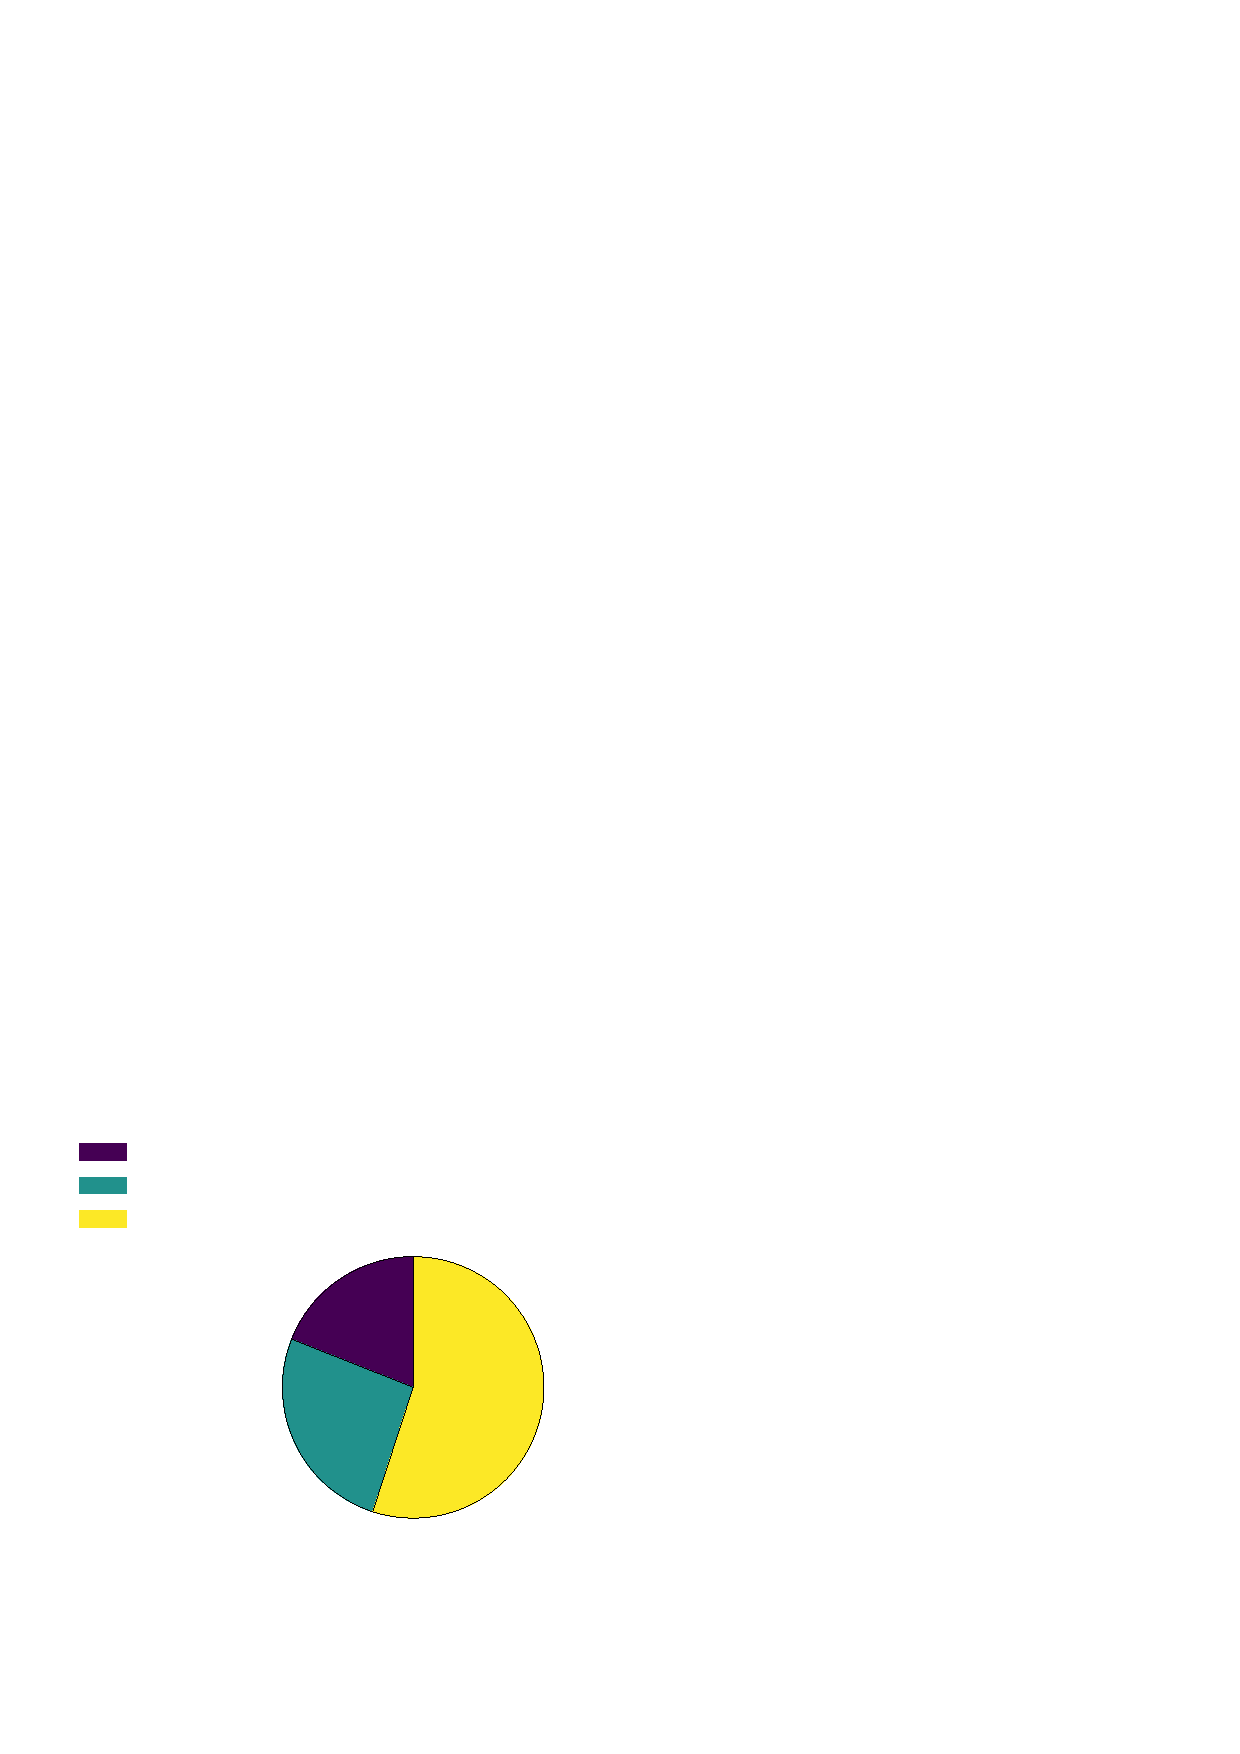
\includegraphics{./figures/parts/01/chapters/01/sections/01/localisation_problems_pie}}%
    \gplfronttext
  \end{picture}%
\endgroup

  \vspace{-2cm}
  \caption{\small Κατάτμηση του προβλήματος της εύρεσης θέσης σε κατηγορίες και
           τα ποσοστά έρευνας σε αυτές}
  \label{fig:localisation_problems_pie}
\end{figure}

Στο μεγαλύτερό της μέρος η παρούσα διατριβή εστιάζει στα δύο πρώτα προβλήματα,
των οποίων η λύση απαιτείται στην πράξη σε κάθε σύστημα με πεδίο εφαρμογής
\ref{scope} που ικανοποιεί την παραδοχή \ref{ass:01_01}.

Δεδομένης της γνώσης του χάρτη του περιβάλλοντος στο οποίο κινείται ένα ρομπότ
κινητής βάσης, της αρχικής και της επιθυμητής του θέσης, ενός αλγορίθμου
παρακολούθησης της θέσης του (pose tracking), και αισθητήρων για την αντίληψη
του περιβάλλοντος, στη γενικότερή του μορφή το πρόβλημα της αυτόνομης πλοήγησης
είναι επιλύσιμο. Για την επίλυσή του απαιτούνται δύο μέθοδοι:

\begin{itemize}
  \item Ένας αλγόριθμος χάραξης μονοπατιού που συνδέει την αρχική με την τελική
        του θέση (Path Planning)
  \item Ένας ελεγκτής κίνησης του ρομπότ για την παρακολούθηση του παραπάνω
        μονοπατιού (Motion Controller)
\end{itemize}


%%%%%%%%%%%%%%%%%%%%%%%%%%%%%%%%%%%%%%%%%%%%%%%%%%%%%%%%%%%%%%%%%%%%%%%%%%%%%%%%
\subsection{Πηγές και κύριοι τρόποι αντίληψης του περιβάλλοντος}

Η επιτυχής λύση του προβλήματος της αυτόνομης πλοήγησης προϋποθέτει την ύπαρξη
και χρήση εξωδεκτικών αισθητήρων. Χωρίς αυτούς τα προβλήματα των οποίων η λύση
είναι αναγκαία για την αυτόνομη πλοήγηση (κατασκευή χάρτη, εύρεση και
παρακολούθηση της θέσης του ρομπότ) δεν είναι επιλύσιμα. Για την αντίληψη των
ορίων (επιφάνειες-εμπόδια) του περιβάλλοντος χρησιμοποιούνται αισθητήρες με
ποικίλα χαρακτηριστικά, ανάλογα με τα χαρακτηριστικά του περιβάλλοντος και
την αντικειμενική επιδίωξη της χρήσης ρομπότ κινητής βάσης. Όσο τα χρόνια
περνούσαν και η τεχνολογία υλικών εκλεπτυνόταν, μαζί της εξελίσσονταν και
οι παραπάνω αλγόριθμοι, οξύνοντας την ακρίβεια εκτίμησης της αναπαράστασης
του περιβάλλοντος χώρου και της θέσης ενός ρομπότ σε αυτό, ή παρέχοντας
περισσότερη και πλουσιότερη πληροφορία για το περιβάλλον.

Τα πρώτα χρόνια της ρομποτικής χρησιμοποιούνταν αισθητήρες υπερήχων (sonar),
εκκινώντας από την ανίχνευση εμποδίων στη γειτονιά ενός ρομπότ. Η τεχνολογία
ήταν εκεί λόγω εκτεταμένης χρήσης τους σε στρατιωτικές επιχειρήσεις, και το
κόστος τους ήταν χαμηλό. Η αρχή λειτουργίας τους βασίζεται στην εκτίμηση
αποστάσεων προς τα γύρω εμπόδια μέσω της μέτρησης του χρόνου εκπομπής υπερήχων
προς και ανάκλασης από αυτά. Αν και χρησιμοποιούνται μέχρι και σήμερα, η χρήση
τους περιορίζεται στην ανίχνευση αντικειμένων σε χαμηλές αποστάσεις λόγω της
αδρής λεπτομέρειας των μετρήσεών τους, το περιορισμένο τους γωνιακό πεδίο
όρασης, και το εγγενές πρόβλημα της αμφισημίας των μετρήσεών τους λόγω των
πολλαπλών διαδοχικών ενδεχόμενων ανακλάσεων του ήχου σε τρίτες επιφάνειες.

Την ίδια αρχή λειτουργίας εκμεταλλεύονται οι αισθητήρες lidar (σύντμηση του
Light και Radar ή αλλιώς Light Detection and Ranging) χρησιμοποιώντας, αντί για
ήχο, φως υπέρυθρης, ορατής, ή υπεριώδους ακτινοβολίας. Διακρίνονται σε
αισθητήρες που αποτυπώνουν αποστάσεις σε εμπόδια του περιβάλλοντός τους σε ένα
επίπεδο (δισδιάστατες μετρήσεις) ή σε πολλαπλά επίπεδα γύρω από αυτό
(τρισδιάστατες μετρήσεις). Οι αισθητήρες LIDAR υστερούν σε κόστος, μέγεθος, και
συχνότητα μετρήσεων σε σχέση με τους αισθητήρες υπερήχων, αλλά εμφανίζουν
σημαντικά μεγαλύτερο εύρος όρασης (έως $360^\circ$), τόσο γωνιακά όσο και
ακτινικά, και ακρίβεια μετρήσεων που μπορεί να φτάσει την τάξη των μερικών
εκατοστών.  Η διαφορά της ακρίβειάς των μετρήσεών τους ως προς την κατασκευή
χάρτη με τη χρήση τους αποτυπώνεται στο σχήμα \ref{fig:sonar_lidar_map}.

\begin{figure}\centering
  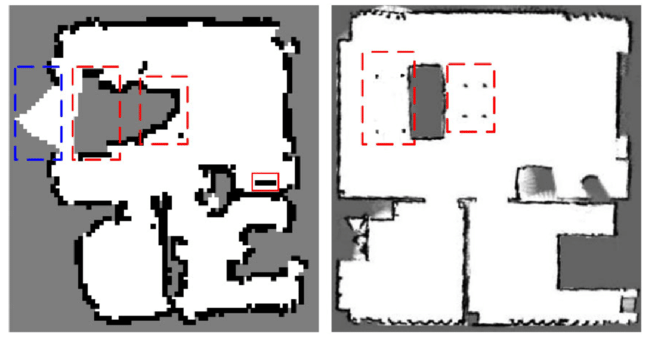
\includegraphics[scale=0.5]{./figures/parts/01/chapters/01/sections/01/sonar_lidar_map.png}
  \caption{\small Αριστερά: δισδιάστατος χάρτης από μετρήσεις αισθητήρα τύπου sonar.
           Δεξιά: χάρτης του ίδιου χώρου από μετρήσεις αισθητήρα τύπου lidar
           σε δύο διαστάσεις \cite{Qi2020}. Τα χρωματισμένα περιγράμματα
           περικλείουν περιοχές τις οποίες ο αισθητήρας sonar απέτυχε να
           χαρτογραφήσει με πιστότητα προς το πραγματικό περιβάλλον}
  \label{fig:sonar_lidar_map}
\end{figure}

Η ανάπτυξη της τεχνολογίας αισθητήρων εικόνας και η βελτίωση της ποιότητάς τους
τούς κατέστησε και πηγές εξωδεκτικών μετρήσεων στη ρομποτική. Το σημαντικό τους
προτέρημα είναι η χρωματική πληροφορία του περιβάλλοντος, το μεγάλο οριζόντιο
και κάθετο εύρος όρασής τους, και ο υψηλός ρυθμός ανανέωσης των μετρήσεών τους.
Η εφεύρεση των αισθητήρων εικόνας και βάθους (RGBD, ή η χρήση στερεοειδών
συστημάτων) εισάγει την επιπρόσθετη πληροφορία κατάληψης σημείων στον
τρισδιάστατο χώρο από εμπόδια, αλλά ταυτόχρονα επιφέρει χαμηλότερες συχνότητες
ανανέωσης αξιοποιήσιμης πληροφορίας λόγω του αυξημένου όγκου της χωρικής πλέον
πληροφορίας. Λόγω του μεγάλου όγκου πληροφορίας που φέρουν απαιτούν
αντίστοιχους υπολογιστικούς πόρους, οι οποίοι στα πλαίσια του πεδίου εφαρμογής
\ref{scope} ενδέχεται να μην είναι διαθέσιμοι. Σε αντίθεση με τους
προηγούμενους αισθητήρες εξαρτώνται από τις συνθήκες φωτισμού του χώρου στον
οποίον λειτουργούν και συνεπώς η ποιότητα των μετρήσεων είναι ευμετάβλητη. Σε
σχέση με τους αισθητήρες lidar εμφανίζουν σημαντικά περιορισμένο γωνιακό εύρος
όρασης, ακρίβεια μετρήσεων που φθίνει τετραγωνικά σε σχέση με την απόσταση
μέτρησης (αντί για γραμμικά όπως στους αισθητήρες lidar), και περιοχές μη
αξιοποιήσιμων μετρήσεων λόγω σκιών που παράγονται ως συνέπεια της αρχής
λειτουργίας τους \cite{Mallick2014}. Η διαφορά της ακρίβειάς των μετρήσεών τους
ως προς την κατασκευή χάρτη με τη χρήση τους αποτυπώνεται στο σχήμα
\ref{fig:rgbd_lidar_map}.

\begin{figure}\centering
  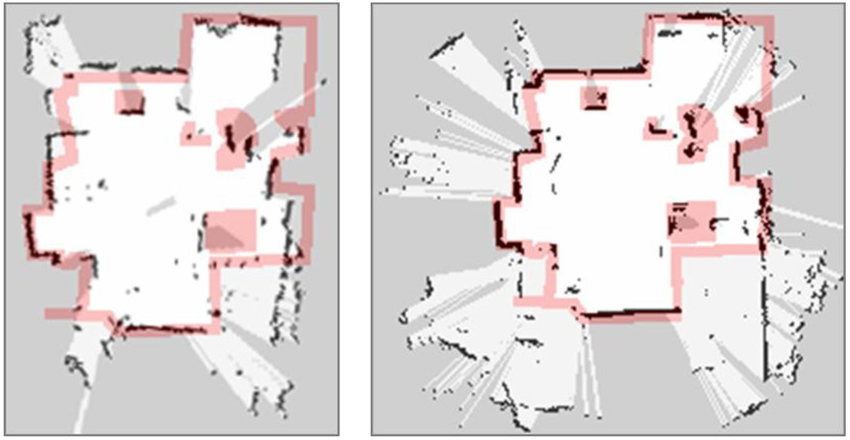
\includegraphics[scale=0.5]{./figures/parts/01/chapters/01/sections/01/rgbd_lidar_map.png}
  \caption{\small Αριστερά: δισδιάστατος χάρτης από μετρήσεις αισθητήρα τύπου
           RGBD προβεβλημένες στο οριζόντιο επίπεδο. Δεξιά: χάρτης του ίδιου
           χώρου από μετρήσεις αισθητήρα τύπου lidar σε δύο διαστάσεις
           \cite{Oliver2012}. Οι κόκκινες γραμμές αναπαραστούν το πραγματικό
           περιβάλλον}
  \label{fig:rgbd_lidar_map}
\end{figure}

Λόγω της μεγάλης τους μετρητικής ακρίβειας, της πυκνής τους γωνιακής
δειγματολειψίας, του ικανού ρυθμού ανανέωσης μετρήσεων, του ευρύτατου πεδίου
οράσεώς τους, του μέτριου κόστους τους, και του γεγονότος ότι ο όγκος των
μετρήσεών τους είναι κατά κύριο λόγο επεξεργάσιμος σε πραγματικό χρόνο
(απαιτητέο από την επίλυση της πλειονότητας των προβλημάτων της υποενότητας
\ref{subsec:01_01_01}), οι αισθητήρες τύπου lidar έχουν προκριθεί στη θέση των
αισθητήρων εκ των ων ουκ άνευ όσο αφορά σε εφαρμογές αυτόνομους πλοήγησης,
κατασκευής χάρτη, και εύρεσης της θέσης ενός ρομπότ, στο πεδίο εφαρμογής
\ref{scope} που ικανοποιούν την παραδοχή \ref{ass:01_01}. Οι ίδιες αρετές τούς
έχουν καταστήσει ηγέτες στην ευρύτερη αγορά αισθητήρων για ρομποτικές εφαρμογές
όπου επιζητείται επιπρόσθετη αντίληψη που να υπηρετεί σκοπούς αυτονομίας (σχήμα
\ref{fig:lidar_share}).


\begin{figure}\centering
  \input{./figures/parts/01/chapters/01/sections/01/lidar_share.eps_tex}
  \caption{\small Αριστερά: κατάτμηση της αγοράς αισθητήρων στην
           αυτοκινητοβιομηχανία \cite{Sighencea2021}. Μέση: πωλήσεις αισθητήρων
           lidar σε εκατομμύρια δολλάρια κατά έτος \cite{statista1}. Δεξιά:
           προβολή της κατάτμησης της αγοράς αισθητήρων και πωλήσεις σε
           δισεκατομμύρια δολλάρια το έτος 2027 \cite{statista2}}
  \label{fig:lidar_share}
\end{figure}


%\begin{bw_box}
%\begin{assumption}
  %\label{ass:01_01_01}
%\end{assumption}
%\end{bw_box}


%%%%%%%%%%%%%%%%%%%%%%%%%%%%%%%%%%%%%%%%%%%%%%%%%%%%%%%%%%%%%%%%%%%%%%%%%%%%%%%%
\subsection{Τρέχουσα κατάσταση και Προκλήσεις}

Τα θεμελιακά προβλήματα που απορρέουν από απαιτήσεις αυτόνομης πλοήγησης,
δηλαδή η κατασκευή χάρτη, η εύρεση και παρακολούθηση της θέσης ενός ρομπότ στο
χώρο, καθώς και η ίδια η αυτόνομη πλοήγηση, θεωρούνται σήμερα λυμένα στο πεδίο
εφαρμογής \ref{scope} με τη χρήση αισθητήρων lidar. Για την ακρίβεια αυτό που
θεωρείται λυμένο είναι το πρόβλημα \textit{επί της αρχής}: δηλαδή ότι υπάρχουν
αναγκαίες συνθήκες στις οποίες η λύση κάθε προβλήματος είναι εφικτή.  Η
αφαίρεση αυτών των συνθηκών και η έρευνα με γνώμονα την ευρωστία στη μετέπειτα
κατάσταση αποτελεί πρόκληση για κάθε μελλοντική λύση.

Επιπρόσθετα η λύση κάθε προβλήματος δεν είναι απαραίτητα ``βέλτιστη".
Παράδειγμα αποτελεί το πεδίο του εντοπισμού της θέσης ενός ρομπότ όπου, λόγω
της παρατήρησης \ref{remark:observable}, η εκτίμηση για τη θέση του φέρει ένα
αναπόφευκτο σφάλμα (λόγω μετρητικού θορύβου και σφαλμάτων μοντελοποίησης και
λύσης).  H ανάγκη για πρόσθετη ή υψηλή ακρίβεια, αν και πάντα ευπρόσδεκτη, δεν
ανήκει στις αυστηρές απαιτήσεις των ρομποτικών εφαρμογών, εκτός από αυτές της
βιομηχανίας.  Στις τελευταίες, ωστόσο, λόγω της ανάγκης για αυστηρές
προδιαγραφές και υψηλή ακρίβεια, η αυτονομία ενός οχήματος είτε αποφεύγεται
(η χειροκίνητη πλοήγηση καθιστά περιττό τον εντοπισμό της θέσης του) είτε,
όπου υιοθετείται, αντικαθίσταται από εξωτερικές και δαπανηρές υποδομές λόγω των
διακυβεύματων που υπάρχουν στο βιομηχανικό πλαίσιο \cite{Vasiljevic2016a}. Σε
αυτό το πλαίσιο αποτελεί πρόκληση η μείωση των σφαλμάτων εκτίμησης της θέσης
ενός ρομπότ, καθώς μικρότερα σφάλματα σημαίνουν περισσότερο γόνιμο έδαφος για
την περαιτέρω αυτοματοποίηση διαδικασιών, και την διεύρυνση υιοθέτησης
ρομποτικών οχημάτων από τη βιοτεχνία/βιομηχανία.


\section{Απαραίτητες έννοιες}
\label{section:01_01_02}
%%%%%%%%%%%%%%%%%%%%%%%%%%%%%%%%%%%%%%%%%%%%%%%%%%%%%%%%%%%%%%%%%%%%%%%%%%%%%%%%
\subsection{Εκτιμητέο διάνυσμα κατάστασης}

Κεντρικής σημασίας στη διατριβή είναι το εκτιμητέο διάνυσμα κατάστασης ενός
επίγειου οχήματος. Μέχρι σε αυτό το σημείο χρησιμοποιείτο αντί αυτής η λέξη
``θέση" για εισαγωγικούς λόγους.

\begin{bw_box}
\begin{definition}
  \textit{Διάνυσμα κατάστασης ή στάση}

Ως διάνυσμα κατάστασης θεωρούμε τη στάση ενός οχήματος στο δισδιάστατο επίπεδο:
τον ειρμό της θέσης του με τον προσανατολισμό του, ως προς το σύστημα αναφοράς
του χάρτη του περιβάλλοντος στο οποίο βρίσκεται το όχημα (σχήμα
\ref{fig:pose_figure}):
  \begin{align}
    \bm{p} = [x \ y \ \theta]^\top
\end{align}

\end{definition}
\end{bw_box}

\begin{figure}[H]\centering
  \input{./figures/01.01.concepts/pose.eps_tex}
  \caption{\small Το διάνυσμα κατάστασης (στάση) $\bm{p} = [x,y,\theta]^\top$
    ενός επίγειου οχήματος στο οριζόντιο επίπεδο}
  \label{fig:pose_figure}
\end{figure}

  Η στάση του οχήματος είναι το αντικείμενο της
  Λόγω παραδοχής \ref{ass:01_01} η στάση είναι

%%%%%%%%%%%%%%%%%%%%%%%%%%%%%%%%%%%%%%%%%%%%%%%%%%%%%%%%%%%%%%%%%%%%%%%%%%%%%%%%
\subsection{Ο αισθητήρας lidar δισδιάστατων μετρήσεων}

\begin{bw_box}
\begin{definition}
  \label{def:lidar}
  \textit{Ορισμός μέτρησης αισθητήρα 2D lidar}

  Μία μέτρηση συμβατικού αισθητήρα 2D lidar αποτελείται από έναν πεπερασμένο
  αριθμό αποστάσεων σε αντικείμενα σε οπτική επαφή εντός της μέγιστης
  εμβέλειάς του. Οι μετρήσεις λαμβάνονται εγκαρσίως προς το σώμα του, σε
  κανονικά γωνιακά και χρονικά διαστήματα, σε ένα καθορισμένο γωνιακό εύρος
  \cite{Cooper2018a}.

  Μία μέτρηση-σάρωση $\mathcal{S}$ που απαρτίζεται από $N_s$ ακτίνες σε γωνιακό εύρος
  $\lambda$ είναι μία διατεταγμένη ακολουθία $\mathcal{S} : \Theta \rightarrow
  \mathbb{R}_{\geq 0}$, όπου
  \begin{align}
  \Theta = \{\theta_n \in [-\frac{\lambda}{2}, +\frac{\lambda}{2}) :
    \theta_n = -\frac{\lambda}{2} + \lambda \frac{n}{N_s},
  n = 0,1,\dots, N_s-1\}
  \end{align}

  Οι γωνίες $\theta_n$ εκφράζονται σε σχέση με τον προσανατολισμό του αισθητήρα
  στο τοπικό του σύστημα συντεταγμένων.
\end{definition}
\end{bw_box}

Το σχήμα \ref{fig:laser} απεικονίζει τη γεωμετρία του ενός τυπικού αισθητήρα
2D lidar, όπου $d_n = \mathcal{S}[-\frac{\lambda}{2} + \frac{\lambda n}{N_s}]$
είναι η απόσταση που αφορά στην ακτίνα με αναγνωριστικό $n$.

\begin{figure}[]\centering
  \definecolor{b}{RGB}{22 38 252}
\begin{tikzpicture}

  \coordinate (O) at (0,0);
  \node (O_n) at (0.2,-0.2) {$O$};
  \node (x_plus) at (3.5,0) {$x$};
  \node (y_plus) at (0,3) {$y$};
  \coordinate (x_minus) at (-2,0);
  \coordinate (y_minus) at (0,-2.5);
  \coordinate (first_ray) at (-2*0.70711, -2*0.70711);
  \coordinate (first_ray_far) at (-2.5*0.70711, -2.5*0.70711);
  \node (ray_0) at (-3.0*0.70711, -3.0*0.70711){ακτίνα $0$};
  \coordinate (last_ray) at (-2*0.70711, 2*0.70711);
  \coordinate (last_ray_far) at (-2.5*0.70711, 2.5*0.70711);
  \node (ray_N) at (-3.0*0.70711, 3.0*0.70711){ακτίνα $N_s$$-$$1$};
  \node (l) at (-1.0,0.2){$\scriptstyle{2\pi-\lambda}$};
  \coordinate(n_c) at (3.0,1.117);
  \node[right] (n_n) at (1.8,1.5){ακτίνα $n$: $\textcolor{b}{d_n = \mathcal{S}[-\dfrac{\lambda}{2} + \dfrac{\lambda n}{N_s}]}$};
  \draw [fill] (n_c) circle [radius=0.05];
  \draw [fill] (O) circle [radius=0.05];
  \node[above] (dn) at (1.0,0.35){$d_n$};

  % draw axes
  \draw [->] (x_minus) -- (x_plus);
  \draw [->] (y_minus) -- (y_plus);
  \draw [dashed] (O) -- (last_ray_far);
  \draw [dashed] (O) -- (first_ray_far);
  \draw [->] (O) -- (n_c);

  % draw laser arc
  \draw [black, thick, dotted] (first_ray) arc[start angle=-135, end angle=135,radius=2];

  % draw 2π - λ arc
  \pic [draw,  angle radius=5mm, angle eccentricity=1.4] {angle = last_ray--O--first_ray};

  % draw n angle arc
  \pic [draw, ->, angle radius=17mm, angle eccentricity=1.4] {angle = x_plus--O--n_c};
  \node (angle_n) at (2.6,0.44){${\scriptstyle-\dfrac{\scriptstyle\lambda}{\scriptstyle 2} + \dfrac{\scriptstyle \lambda n}{\scriptstyle N_s}}$};

\end{tikzpicture}

  \caption{\small Κάτοψη του τοπικού συστήματος αναφοράς ενός τυπικού αισθητήρα
           αποστάσεων τύπου lidar. Ο αισθητήρας είναι τοποθετημένος στο $O(0,0)$
           και ο προσανατολισμός του είναι αυτός του θετικού $x$ άξονα. Το
           γωνιακό πεδίο οράσεώς του είναι $\lambda$}
  \label{fig:laser}
\end{figure}

\begin{bw_box}
\begin{definition}
  \textit{Πανοραμικός αισθητήρας 2D lidar}

  Το γωνιακό εύρος ενός 2D lidar είναι συμμετρικά κατανεμημένο ως προς τον
  τοπικό του $x$ άξονα. Κάθε ακτίνα έχει την ίδια γωνιακή απόσταση από τις
  γειτονικές της, εξαιρέσει των δύο ακραίων ακτίνων όταν $\lambda < 2\pi$.
  Όταν $\lambda = 2\pi$ ο αισθητήρας ονομάζεται πανοραμικός.
\end{definition}
\end{bw_box}

%%%%%%%%%%%%%%%%%%%%%%%%%%%%%%%%%%%%%%%%%%%%%%%%%%%%%%%%%%%%%%%%%%%%%%%%%%%%%%%%
\subsection{Το φίλτρο σωματιδίων}
%%%%%%%%%%%%%%%%%%%%%%%%%%%%%%%%%%%%%%%%%%%%%%%%%%%%%%%%%%%%%%%%%%%%%%%%%%%%%%%%
\subsection{Ευθυγράμμιση σαρώσεων lidar}
%%%%%%%%%%%%%%%%%%%%%%%%%%%%%%%%%%%%%%%%%%%%%%%%%%%%%%%%%%%%%%%%%%%%%%%%%%%%%%%%
\subsection{Τα προβλήματα εύρεσης στάσης}
%%%%%%%%%%%%%%%%%%%%%%%%%%%%%%%%%%%%%%%%%%%%%%%%%%%%%%%%%%%%%%%%%%%%%%%%%%%%%%%%
\subsection{Το λειτουργικό σύστημα ρομπότ ROS}

